\documentclass[]{book}
\usepackage[english]{babel}
\usepackage{graphicx}
\usepackage{amsmath}
\usepackage{cite}
\usepackage{hyperref}
\usepackage{caption}



\begin{document}

\chapter*{Data Acquisition System }

\noindent La medición constituye un pilar fundamental de la investigación científica. Sin embargo, la cuantificación de una magnitud física solo se puede llevar a cabo a través de la interacción con el sistema y la extracción de la información de interés. A partir de estos conceptos es posible enmarcar la guía del presente capítulo, explorando los métodos que permiten convertir fenómenos físicos en señales que transporten información y las tecnologías que hacen posible la adquisición de dichas señales y su representación en un formato útil para el observador o  usuario \cite{webster2018measurement}. El conjunto de procesos diseñados para extraer información de un sistema físico se denomina sistema de adquisición de datos e incluye varias etapas que se ilustran en la figura \ref{fig:DAQ_generic} y se describen a continuación.\\

\begin{figure}[h]
    \centering
    
\includegraphics[width=1.0\textwidth]{DAQ_chain.png}
    \caption{Diagrama de los principales componentes de un sistema de adquisición de datos genérico}
    \label{fig:DAQ_generic}

\end{figure}

\noindent En primer lugar, es fundamental identificar un sistema de interés y las variables que se desean medir. Cualquier objeto físico puede ser estudiado siempre que se cuente con el marco teórico y los métodos experimentales adecuados para extraer sistemáticamente sus medidas. Por ejemplo, si se considera el universo observable, es posible medir su tasa de expansión mediante argumentos cosmológicos y un sistema de telescopios que observe cambios en las características de la luz proveniente de diversas galaxias, lo que evidencia la expansión del universo \cite{weinberg1976first}. Por otro lado, un tumor cerebral puede evaluarse al analizar los cambios en los espines nucleares de los átomos de hidrógeno en los tejidos cerebrales al aplicar un campo magnético potente para alinear estos espines, y luego pulsos de radiofrecuencia para perturbar esta alineación. La respuesta de los espines al campo magnético y a los pulsos de radiofrecuencia se detecta y se utiliza para crear imágenes detalladas de los tejidos cerebrales \cite{ernst1990principles}. Aunque estos ejemplos pueden parecer desconectados, comparten un elemento clave: son sistemas físicos cuyos atributos pueden medirse mediante la interacción con un medio capaz de extraer información. \\

\noindent El medio mencionado es diseñado sistemáticamente para interactuar con el objeto de interés. Estos medios son comúnmente dispositivos llamados sensores, un tipo de transductor capaz de convertir estímulos físicos en señales, generalmente eléctricas. Como se ha mencionado, existe una amplia variedad de sensores diseñados para medir todo tipo de magnitudes físicas, los cuales explotan distintos fenómenos en función de los requisitos de la medición \cite{webster2018measurement}. Por ejemplo, para medir la temperatura de un objeto, se pueden utilizar aleaciones metálicas que cambian su resistividad eléctrica ante variaciones de temperatura \cite{scarr1960thermistors}. Sin embargo, una cámara fotosensible al espectro infrarrojo también podría cumplir la misma función \cite{driggers2012introduction}. Estos sistemas se diferencian en la metodología con la que la información de los cambios de temperatura es transferida al usuario. En el primer caso, se requiere la lectura de la resistividad eléctrica y el conocimiento de su tasa de cambio en función de la temperatura, mientras que en el segundo caso, se emplea un sistema óptico equipado con la tecnología necesaria para convertir la radiación electromagnética en señales eléctricas. Finalmente estas señales pueden ser manipuladas para calcular la temperatura del objeto original utilizando la ley de Planck \cite{krane2019modern}.\\

\noindent Para lograr la extracción y transferencia efectiva de información hacia el observador, esta debe ser presentada en un formato que permita su codificación, transporte y almacenamiento sin pérdidas. En este contexto, las señales eléctricas, y por ende los dispositivos electrónicos, desempeñan un papel crucial en los sistemas modernos de adquisición de datos. Estos sistemas integran tanto componentes analógicos como digitales en sus diferentes etapas, tal como se ilustra en la figura \ref{fig:DAQ_generic}. \\

\noindent En general, las señales provenientes del sensor o detector deben ser tratadas y acondicionadas según las características que se deseen resaltar y preservar. Por ejemplo, es común que factores externos e internos de los sistemas electrónicos introduzcan señales no deseadas, conocidas como ruido, en la señal de interés, lo que hace necesario el uso de filtros de frecuencia o amplitud. Además, puede ocurrir que la señal generada por el sensor sea muy débil y las etapas subsecuentes no tengan la resolución adecuada para procesarla, por lo que se deben implementar amplificadores de distintos tipos. En otros casos, es necesario transformar el tipo de señal que transporta la información, por ejemplo, de carga a voltaje o de voltaje a corriente. Estas tareas suelen ser realizadas por circuitos de dispositivos analógicos, conocidos como etapas de acondicionamiento de señales, que algunos autores denominan analog front-end \cite{kledrowetz2023fully}.\\

\noindent Sin embargo, ante grandes volúmenes de datos, se requieren sistemas de cómputo con la capacidad de manejar señales con alta precisión, almacenar datos sin degradación y ejecutar operaciones complejas a gran velocidad, predominando los circuitos digitales como la tecnología principal en este ámbito. Como resultado, las etapas de procesamiento en los sistemas de adquisición de datos (DAQ) modernos están generalmente basadas en esta tecnología. Estos sistemas utilizan señales discretas, que representan información en forma de bits (0s y 1s), en contraste con las señales analógicas continuas. Como se mencionó anteriormente, estos sistemas aplican sobre las señales diversas operaciones, que pueden incluir clasificación, discriminación y la ejecución de operaciones matemáticas. Entre los principales exponentes de la electrónica digital se encuentran plataformas como procesadores o CPUs, FPGAs, ASICs, GPUs, DSPs, SoCs y computadoras cuánticas. Cada una de estas plataformas posee características únicas que las hacen especialmente adecuadas para diversas aplicaciones en el procesamiento de datos \cite{proakis2007digital}.\\

\noindent Si bien las plataformas mencionadas pueden ejecutar operaciones en linea, es decir, procesan las señales en la medida que ingresan al sistema, es necesario enviar la información a etapas externas del DAQ para llevar a cabo actividades como el almacenamiento, posprocesamiento, interacción con otros sistemas de detección (trigger) y transferencia a interfaces de alto nivel de abstracción como las computadoras de escritorio, para que el usuario pueda acceder a ella. Dependiendo de la complejidad de la aplicación y por ende del DAQ, distintos tipos de interfaces de comunicación pueden ser utilizados. Algunos ejemplos de estos protocolos, abarcando desde tecnología de consumo hasta grandes distribuciones de servidores son: RS-232, RS-485, USB, GPIB, Ethernet, Wi-Fi, Modbus/TCP, CAN Bus, Profibus, Profinet, SCADA, EtherCAT, MMS, MQTT, OPC UA, LHC Computing Grid, INFN-Tier-1 \cite{zurawski2014industrial} \cite{bortolotti2012infn}.\\

\noindent Finalmente, mediante el uso de programas informáticos diseñados específicamente para decodificar los datos provenientes de la interfaz de comunicación, las cantidades físicas de interés pueden presentarse en formatos comprensibles y útiles para el usuario. Por ejemplo, un osciloscopio que transmite datos a una computadora de escritorio a través de una interfaz GPIB-USB cuenta con una interfaz gráfica de usuario que permite visualizar la señal en el dominio del tiempo, destacando características como amplitud, frecuencia, y valor de la línea base. De manera similar, un sistema de espectroscopía nuclear puede enviar datos a través de Ethernet a un servidor, donde estos se almacenan en una base de datos accesible para usuarios de la red \cite{crespo2021remote}. Con aplicaciones web, es posible generar histogramas de energía frente a la altura, visualizando así los espectros de energía de una fuente de radiación. En última instancia, el objetivo de cualquier sistema de adquisición de datos, independientemente de su escala o infraestructura, es proporcionar al usuario información física relevante para su análisis e interpretación.\\

\noindent A continuación, se presentarán algunos conceptos clave sobre los sistemas de Adquisición de Datos (DAQ) con el propósito de profundizar en las características de sus etapas generales y establecer una base sólida para abordar el DAQ desarrollado en este trabajo. Posteriormente, se describirá el montaje experimental y la metodología empleada para su implementación.\\

\section{Marco Teórico}
\subsection{Sensores y Detectores}

\noindent Como se expuso anteriormente, un sensor es un dispositivo que responde a un estímulo físico, químico o biológico específico, y genera una señal correspondiente, generalmente de tipo eléctrico, que tiene una relación funcional con la magnitud del estímulo. Los sensores suelen estar compuestos por dos componentes principales: el elemento sensible o transductor, que interactúa directamente con el estímulo (por ejemplo, temperatura, presión, luz) y un mecanismo de conversión que traduce la respuesta del transductor en una señal utilizable (como una corriente o voltaje eléctrico). La precisión, sensibilidad, resolución y rango de operación son características clave que determinan el rendimiento de un sensor \cite{webster2018measurement}.\\

\noindent Los sensores se pueden clasificar según diversos criterios: por el tipo de magnitud que miden, el principio de funcionamiento (resistivos, capacitivos, inductivos, piezoeléctricos), el tipo de señal de salida (analógicos, digitales), la forma de operación (activos, pasivos), y la naturaleza del contacto con la magnitud medida (de contacto, sin contacto). Además, según su contexto de uso, los sensores pueden ser clasificados como domésticos (utilizados en electrodomésticos y dispositivos de consumo), industriales (empleados en automatización y control de procesos), o científicos (destinados a investigación y aplicaciones especializadas) \cite{sinclair2000sensors}.\\

\noindent En particular, estos últimos destacan por su alta precisión, exactitud, sensibilidad, robustez y fiabilidad. Su objetivo es proporcionar mediciones extremadamente precisas y reproducibles, ya que los resultados son cruciales para investigaciones avanzadas. Además, suelen poseer un amplio rango dinámico, lo que les permite detectar tanto variaciones muy pequeñas como extremadamente grandes en las magnitudes de interés. Un ejemplo destacado en este grupo son los detectores de radiación o partículas, que sobresalen por su capacidad para interactuar con corpúsculos a nivel atómico y subatómico, generando señales pulsadas que revelan propiedades esenciales de las partículas incidentes, como su energía, momento lineal o trayectoria, entre otras \cite{knoll2010radiation}. Existen diferentes tipos de detectores de partículas, cada uno optimizado para aplicaciones específicas. Los detectores de estado sólido, como los semiconductores de silicio, son ampliamente utilizados por su alta resolución espacial y temporal. Estos dispositivos funcionan mediante la creación de pares electrón-hueco cuando una partícula cargada atraviesa el material, generando una señal eléctrica proporcional a la energía depositada. Por otro lado, los detectores gaseosos, como las cámaras de ionización o los contadores proporcionales, operan en medios gaseosos donde la ionización del gas produce electrones libres y iones positivos que se colectan para formar una señal. Estos detectores son valiosos por su capacidad para cubrir grandes volúmenes, lo que es esencial en experimentos que requieren la detección de partículas en áreas extensas. Además, existen otros tipos de detectores como los cintiladores, que emiten luz cuando son excitados por radiación ionizante, y los detectores Cherenkov, que detectan partículas cargadas moviéndose a velocidades superiores a la velocidad de la luz en un medio dado \cite{kolanoski2020particle}.



\subsection{Señales Eléctricas de Sensores}

\noindent Dado que las señales eléctricas son esenciales en este contexto como portadoras de la información física que se busca extraer, es fundamental describir sus principales características para comprender cómo las etapas electrónicas del sistema de adquisición de datos (DAQ) las afectan. Aunque las señales pueden ser digitales o análogas, generalmente las producidas por un sensor o detector son de tipo análogo. \\

\noindent Una señal analógica proveniente de un sensor se caracteriza principalmente por su variación continua en el tiempo y su capacidad para representar información en un rango infinito de valores. La amplitud de la señal refleja la magnitud del parámetro medido, como temperatura o presión, y puede variar suavemente en respuesta a cambios en el entorno. La frecuencia de la señal puede no ser relevante en todos los casos, pero el tiempo de respuesta y la estabilidad son cruciales para asegurar mediciones precisas. Además, la señal puede estar afectada por ruido y errores, lo que requiere técnicas de filtrado y calibración para obtener datos confiables. La forma de onda de la señal es continua y puede ser analizada en el dominio del tiempo para evaluar su comportamiento y en el dominio de la frecuencia para identificar componentes relevantes \cite{sinclair2000sensors}. En la figura \ref{fig:generic_signal}, se ilustra una señal en el dominio del tiempo proveniente de un sensor de aceleración.\\

\begin{figure}[h]
    \centering
    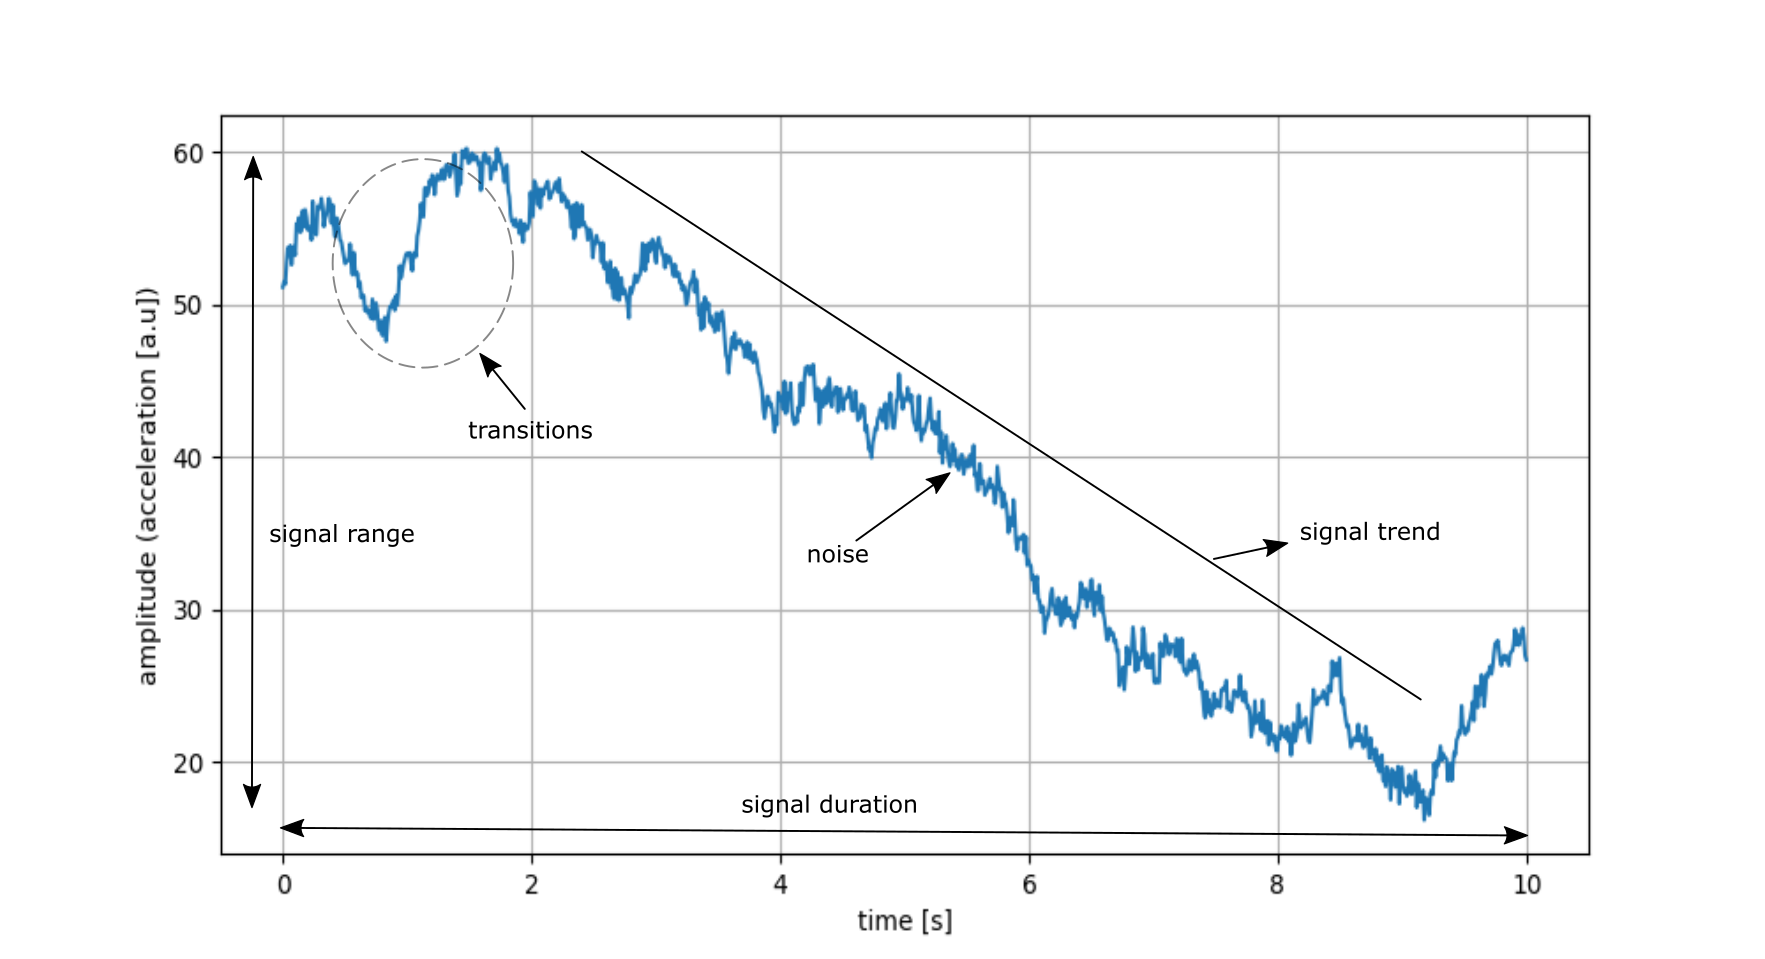
\includegraphics[width=0.8\textwidth]{mysignal.png}
    \caption{Señal no periódica en el dominio del tiempo proveniente de un sensor de aceleración. En ella es posible observar algunas características como duración, rango de la magnitud de interés en el lapso registrado, ruido electrónico, tendencia y transitorios. La amplitud de la señal solo puede ser definida con base a un nivel de referencia.}
    \label{fig:generic_signal}

\end{figure}

\noindent Un caso de particular interés son las señales producidas por los detectores de partículas, que en general son de naturaleza pulsada. En este contexto, se puede asociar la detección de un evento con una perturbación, denominada pulso, que se define sobre la línea base de la señal de salida. La figura \ref{fig:pulse} muestra un ejemplo genérico de un pulso individual, utilizado para ilustrar algunas de sus características principales.

\begin{figure}[h]
    \centering
    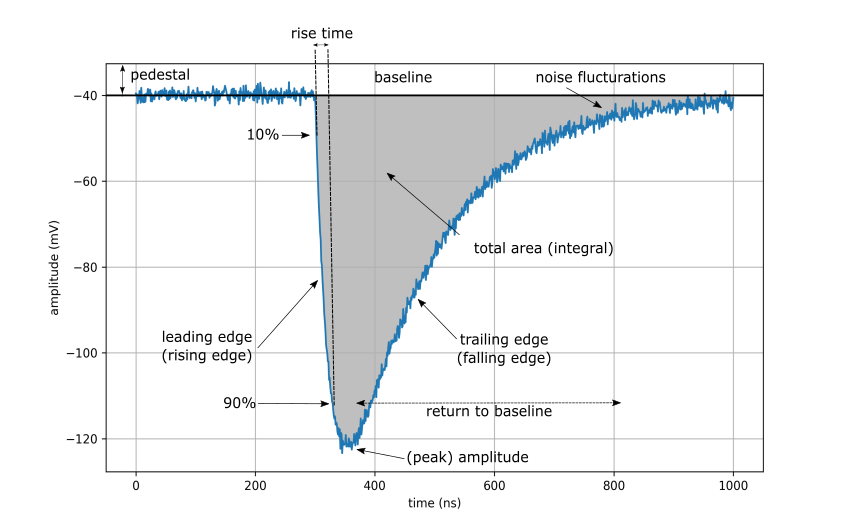
\includegraphics[width=1.0\textwidth]{pulse_edited.png}
    \caption{Pulso típico genérico para ilustrar las principales características. Reproducido a partir de \cite{kolanoski2020particle}}
    \label{fig:pulse}

\end{figure}

\noindent Según \cite{knoll2010radiation}, suponiendo que la señal generada por el detector es corta comparado con los tiempos típicos de procesamiento de la electrónica de lectura, las cantidades que caracterizan un pulso son:

\begin{itemize}
    \item La amplitud máxima del pulso: también conocida como altura del pulso, es el valor máximo que alcanza la señal. En sistemas lineales, este valor es proporcional a la energía primaria depositada en el detector.
    \item Tiempo de pico: Es el momento en el tiempo en el que se alcanza la amplitud máxima del pulso.
    \item Área o integral del pulso: Representa el área bajo la curva del pulso. En sistemas lineales y para señales cortas tipo $\delta$, su valor debería ser proporcional a la energía primaria depositada.
    \item Ancho del pulso: Se refiere a la duración del pulso, que generalmente se define como el ancho total a la mitad de la altura máxima (FWHM, por sus siglas en inglés).
    \item Bordes de subida y bajada: Son las pendientes ascendente y descendente del pulso.
    \item Tiempo de subida: Caracteriza la rapidez con la que el pulso aumenta. Comúnmente se define como el tiempo necesario para que el pulso pase del 10\% al 90\% de su amplitud máxima, aunque existen otras definiciones.
    \item Tasa de variación (Slew rate): Indica el cambio de voltaje por unidad de tiempo $dV/dt$ y se expresa en unidades de $V/s$.
    \item Línea base o valor de pedestal: Es el valor de salida cuando no hay ninguna señal de entrada. Define el nivel 'cero' desde el cual se mide la altura de la señal. Aunque generalmente la línea base tiene un valor fijo, pueden ocurrir desviaciones durante un cierto (y breve) período de tiempo. Estas desviaciones se conocen como desplazamientos de la línea base.
    \item Tiempo de retorno a la línea base: Es el tiempo necesario para que la amplitud del pulso vuelva al valor de la línea base.
    \item Suboscilación: Se refiere a la parte de la amplitud de un pulso que tiene un signo opuesto (con respecto a la línea base) en comparación con la amplitud principal.
    \item Señal unipolar: Es una forma de pulso en la que, salvo por las fluctuaciones de ruido, el valor de la amplitud se mantiene por encima o por debajo de la línea base en todo momento $t$. Por lo general, también se incluyen en esta definición las señales con pequeñas suboscilaciones.
    \item Señal bipolar: Es una forma de pulso en la que la parte del pulso que ocurre más tarde en el tiempo tiene un signo opuesto al de la parte que ocurre primero.
\end{itemize}

\noindent Por otro lado, las señales digitales, esenciales en el procesamiento de información, se caracterizan por su naturaleza discreta tanto en el tiempo como en la amplitud, en tanto que solo pueden adoptar dos estados, representados por los valores 1 y 0. Es de resaltar, que las señales analógicas tratadas anteriormente, son convertidas a digitales mediante un dispositivo denominado conversor análogo digital o ADC. Adicionalmente. a partir de una señal digital base con frecuencia constante, conocida como reloj, se puede codificar información en señales digitales mediante código binario y operaciones de conteo. Básicamente, se mide cuántos ciclos de reloj la señal permanece en un estado u otro. Esta metodología es altamente versátil, ya que permite realizar operaciones matemáticas utilizando el sistema binario \cite{brown2000fundamentals}. En la figura \ref{fig:digital_siganl} se puede observar un ejemplo de señal digital para ilustrar.

\begin{figure}[h]
    \centering
    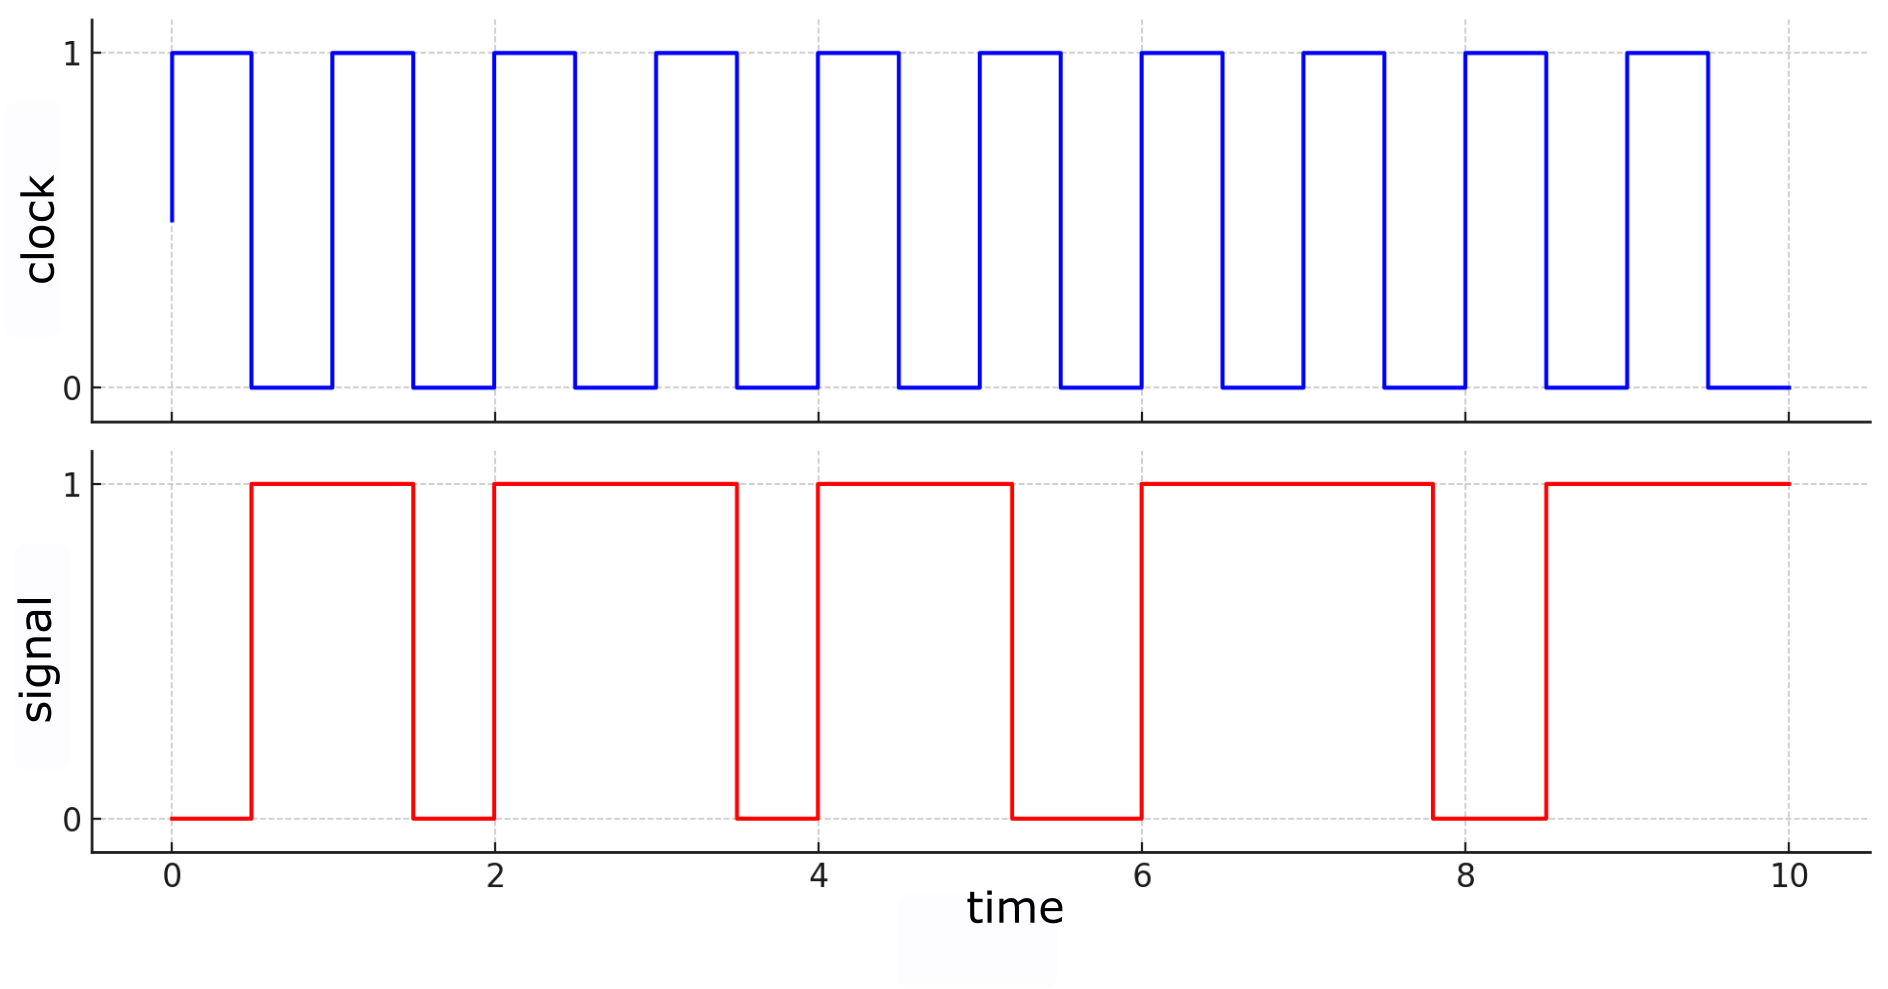
\includegraphics[width=0.7\textwidth]{digital_signal.png}
    \caption{Ejemplo de diagrama de tiempo de una señal digital. En la parte superior se muestra una señal típica de reloj y en la parte inferior una señal genérica con información codificada en su estado (ampitud) o en su duración (ancho).}
    \label{fig:digital_siganl}

\end{figure}

\section{Tratamiento y acondicionamiento de Señales}

\noindent Próxima al sensor, se encuentra la etapa de tratamiento y acondicionamiento, que típicamente comprende electrónica analógica para la amplificación, shaping y digitalización de la señal. Esta etapa es esencial para filtrar y modular la señal, otorgándole las características adecuadas para ser transferida a las etapas de procesamiento digital posteriores. En la figura \ref{fig:generic_frontend} se observa un esquema genérico de esta sección de la cadena de adquisición de datos.\\

\begin{figure}[h]
    \centering
    
\includegraphics[width=0.8\textwidth]{front-end.png}
    \caption{Un esquema de una etapa de electrónica de acondicionamiento típico, utilizado a menudo para la lectura de un detector, que incluye amplificación, conformación de impulsos y digitalización (representada aquí por un ADC).}
    \label{fig:generic_frontend}

\end{figure}

\noindent Los sistemas involucrados en esta etapa, deben cumplir con tres características: (a) ser causales, (b) invariantes en el tiempo, y (c) lineales al menos en la primera etapa de amplificación. Un sistema se considera causal si, en cualquier momento, solo depende del valor de su entrada en ese instante. Es invariante en el tiempo si la relación entre la salida y la entrada, por ejemplo, el ratio $\text{señal}_{\text{entrada}}/\text{señal}_{\text{salida}}$ no varía con el tiempo \cite{kolanoski2020particle}. La linealidad del sistema implica que la señal de salida (por ejemplo, $v_{out(t)}$) no depende del tamaño de la señal de entrada (por ejemplo, $i_{in(t)}$), esto es, 

$$
v_{\text {out }}\left(\alpha \times i_{\text {in }}(t)\right)=\alpha \times v_{\text {out }}\left(i_{\text {in }}(t)\right)
$$

\noindent En muchos casos, la magnitud a la salida de un sensor puede ser muy pequeña, por lo que es necesario implementar etapas de preamplificación y amplificación que aumenten la amplitud de la señal (ganancia) hasta que esta se encuentre en el rango de sensibilidad de las etapas posteriores. Para llevar a cabo tal función, es posible utilizar dintintos dispositivos, sin embargo, los más comunes son los amplificadores operacionales y transistores. Usualmente las señales de entrada provenients del sensor o detector al preamplificador son transformadas en señales de voltaje $(V)$ o de corriente $(I)$. Dependiento de los tipos de entrada y salida, es posible distinguir \cite{kolanoski2020particle}:

\begin{itemize}
    \item amplificador de voltaje: $V \rightarrow V$,
    \item amplificador de corriente: $I \rightarrow I$,
    \item amplificador de transconductancia: $V \rightarrow I$,
    \item amplificador de transimpedancia: $I \rightarrow V$,
    \item amplificador de carga: $Q \rightarrow V$ (o $I$).
\end{itemize}

\noindent Como expone \cite{knoll2010radiation}, La función principal del preamplificador es captar la señal del detector sin deteriorar notablemente la SNR inherente. Por ello, el preamplificador se ubica generalmente lo más cerca posible del detector para reducir la carga capacitiva $(C)$ sobre este. Por ejemplo, un preamplificador de voltaje amplifica directamente la señal de voltaje $V_{\text{in}}$, manteniendo una alta impedancia de entrada $Z_{\text{in}}$ y una baja impedancia de salida $Z_{\text{out}}$ para asegurar una transferencia eficiente y reducir la influencia del ruido. En ambos casos, la linealidad del preamplificador es crucial para que la relación $V_{\text{out}}/ V_{\text{in}}$ se mantenga constante, lo cual es esencial para la precisión en la medición \cite{leo1994techniques}.\\

\noindent Por otro lado, un preamplificador de carga convierte una señal de carga $Q$ generada por el detector en un voltaje proporcional $V$, dada la relación: 

\begin{equation}
    V = \frac{Q}{C}
\end{equation}

La figura \ref{fig:preamp} ilustra su comportamiento típico sobre la señal del detector.\\

\begin{figure}[h]
    \centering
    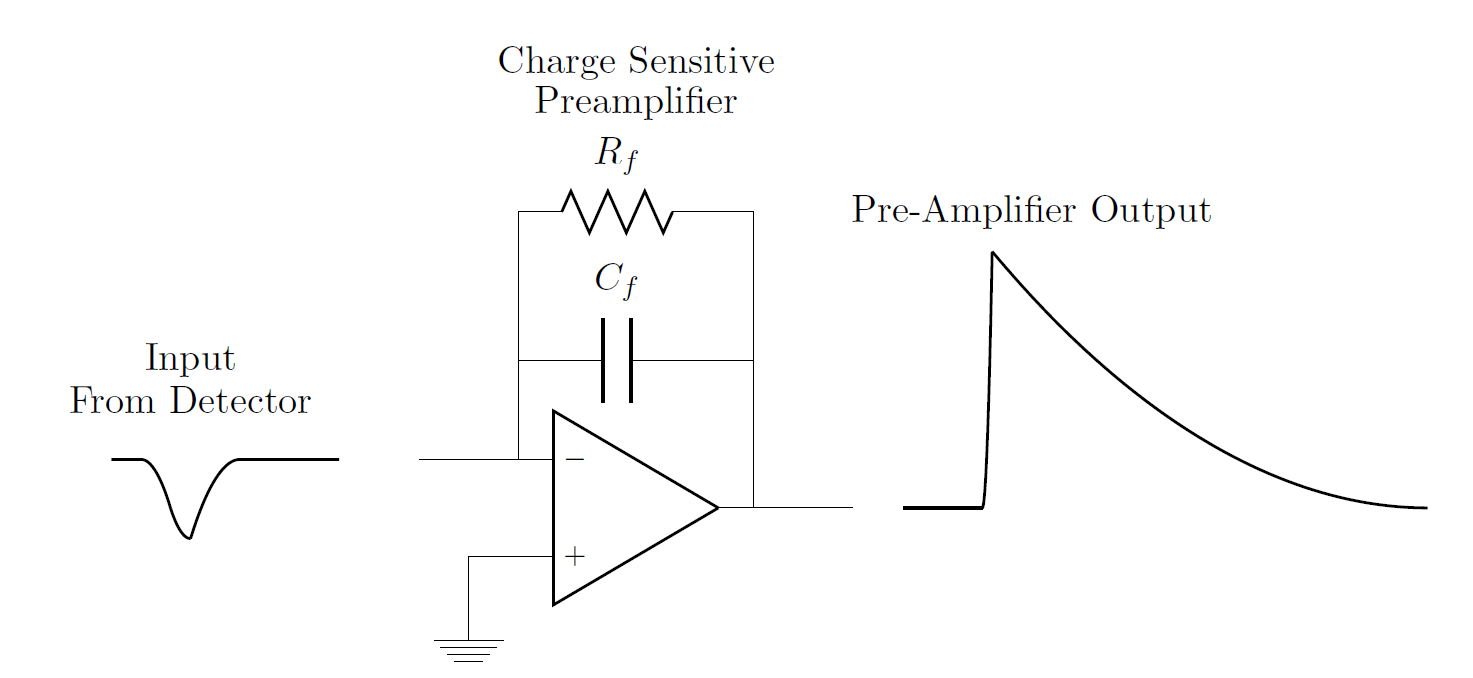
\includegraphics[width=0.8\textwidth]{preamp.PNG}
    \caption{Ilustración del comportamiento de un preamplificador de carga. Este tipo de dispositivos son comúnmente utilizados para acondicionar señales pulsadas provenientes de detectores de partículas \cite{kolanoski2020particle}.}
    \label{fig:preamp}

\end{figure}

\noindent Como explica \cite{webster2018measurement}, la amplificación por etapas de una señal ofrece numerosas ventajas significativas. Principalmente, permite reducir el ruido generado en cada etapa individual, resultando en una señal final más limpia y menos propensa a la distorsión. Este método también mejora la estabilidad del sistema al distribuir la amplificación, evitando la saturación que podría ocurrir con una amplificación intensa en una sola etapa. Además, facilita el control preciso de la ganancia y la adaptación de impedancias entre diferentes componentes, lo cual mejora la eficiencia y la transferencia de la señal. La amplificación gradual es particularmente útil para manejar señales débiles, amplificándolas sin riesgo de distorsión. Asimismo, distribuye la carga térmica generada, disminuyendo el riesgo de sobrecalentamiento de los componentes. \\

\noindent La etapa de amplificación principal generalmente se realiza mediante un amplificador operacional con una resistencia en realimentación. Como modelo matemático, el detector, representado como una capacitancia a descargar, suministra la señal de corriente $i_{s}$ a través de la resistencia $R_{s}$ a un nivel de referencia en un tiempo $\Delta t$. Si el tiempo de descarga es grande comparado al tiempo de duración de la señal 

\begin{equation}
    \left(\tau=R_S C_D \gg\right. \Delta t)
\end{equation}

en cierto sentido, el detector integra la señal de corriente en la capacitancia del detector 

\begin{equation}
    \left(V_D=Q_S / C_D\right) 
\end{equation}

y a la entrada del amplificador se tiene el voltaje 

\begin{equation}
    v_{\text{in}}(t)=V_D \exp \left(-t / R_S C_D\right)
\end{equation}

\noindent El voltaje de salida es proporcional a $v_{i n}$ y el sistema opera como un amplificador de voltaje \cite{kolanoski2020particle}:


\begin{equation}
    v_{\text {out }}(t)=-\frac{R_f}{R_S} v_{\text {in }}(t)=-\frac{R_f V_D}{R_S} \exp \left(-t / R_S C_D\right) .
\end{equation}


\subsubsection{Signal Shaping}

\noindent En la cadena de tratamiento de señales, la etapa de shaping es un circuito electrónico fundamental que modifica la forma de una señal para optimizar su calidad y adaptarla a los requisitos del procesamiento subsiguiente. Generalmente, esta etapa se integra en la fase de preamplificación o amplificación, y es especialmente relevante en sistemas de detección de partículas. Su función principal es transformar señales pulsadas, que pueden presentar formas diversas, en pulsos uniformes y bien definidos. Esta uniformidad es crucial para evitar la superposición de pulsos (pile-up) y disminuir el ruido mediante un filtrado de frecuencia eficiente \cite{leo1994techniques}.\\

\noindent Los pulsos electrónicos generados por el preamplificador tienen tiempos de decaimiento típicos que varían entre unos pocos nanosegundos y varios microsegundos. Si llegan señales adicionales durante el tiempo de decaimiento, puede ocurrir pile-up a pesar de que el capacitor de retroalimentación del preamplificador se descargue. Para mitigar esto, se utilizan filtros pasa-altos y pasa-bajos, que permiten separar las señales superpuestas y moldear los pulsos de salida en formas más Gaussianas. Además, los filtros ayudan a reducir el ruido blanco que afecta a todas las frecuencias, mejorando así la SNR \cite{kolanoski2020particle}. La figura \ref{fig:shaper} ilustra las formas de pulsos típicos en la salida del preamplificador que ingresan una configuración de shaping básica compuesta por un circuito CR-RC. Usualmente se observa una caída (undershoot) en la salida del shaper, la cual se corrige con la cancelación polo-cero\footnote{Técnica de diseño de circuitos que anula efectos indeseados al colocar un cero en la misma frecuencia que un polo, mejorando la respuesta del sistema.} \\

\begin{figure}[h]
    \centering
    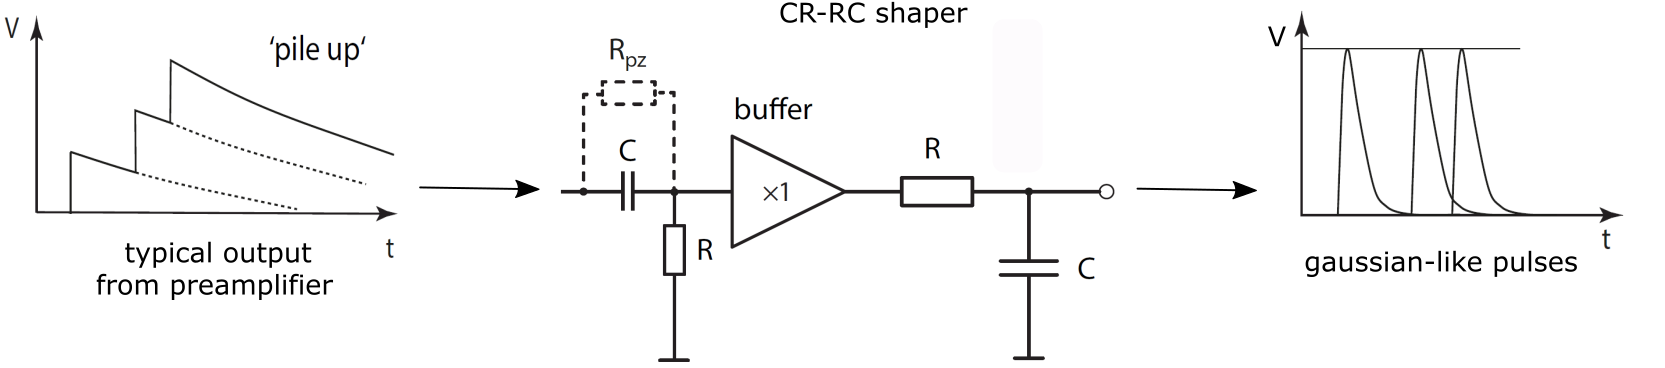
\includegraphics[width=1.0\textwidth]{shaper_chain.png}
    \caption{Funcionamiento típico de un shaper. La resistencia $R_{\text{pz}}$ paralela al condensador del filtro de paso alto se utiliza para la corrección del undershooting. El amplificador (×1) entre las secciones del filtro de paso de banda sirve como un buffer, impidiendo que el filtro de paso bajo aplique una carga significativa al filtro de paso alto. Adaptado de \cite{kolanoski2020particle}.}
    \label{fig:shaper}
\end{figure}

\noindent Es importante destacar que el proceso de shaping puede realizarse en la etapa de procesamiento digital, según los requisitos específicos de la aplicación. Formas de pulso, como la trapezoidal, que son difíciles de generar mediante electrónica analógica, pueden implementarse de manera más eficiente en el dominio digital mediante filtros con parámetros ajustados en plataformas configurables como las FPGA \cite{radeka1968optimum}. Este enfoque se explorará con mayor detalle en la sección \ref{sec:digital_processing}.\\


\subsubsection{Digitalización}

\noindent De acuerdo con \cite{meyer2007digital}, la digitalización de las señales provenientes de sensores es crucial debido a la precisión y flexibilidad que ofrece frente a los métodos analógicos tradicionales. Con el avance de los convertidores analógico-digitales (ADC) de alta velocidad y buena resolución desde los años 90, la posibilidad de procesar digitalmente las señales de los sensores se ha consolidado.\\

\noindent Las ventajas de este enfoque incluyen una flexibilidad ilimitada en la elección de parámetros de procesamiento, mayor estabilidad al eliminar el riesgo de derivas debido a cambios de temperatura o voltaje, y la capacidad de realizar análisis más detallados con múltiples salidas de un mismo sensor. Además, la manipulación digital no introduce ruido adicional y permite la implementación precisa de formas de señal que serían difíciles o imposibles de lograr en circuitos analógicos. Sin embargo, una desventaja potencial es la limitación en la precisión temporal, ya que los sistemas digitales están restringidos a la frecuencia de muestreo más cercana, lo que puede ser menos exacto que los métodos analógicos en aplicaciones que requieren una temporización muy rápida.\\

\noindent La función principal de un ADC es generar un código digital o número en su salida, que sea proporcional a la tensión analógica suministrada a su entrada, realizando las conversiones de forma continua a una frecuencia de reloj fija. Por ejemplo, un reloj de 500 MHz producirá 500 MSPS (Megasamples per Second), lo que equivale a una muestra cada 2 ns. \\

\noindent La resolución del ADC, que se determina por el número de bits del convertidor, afecta directamente a la precisión de estas conversiones. Un número binario con $n$ bits puede representar $2^{n}$ valores. Durante la digitalización, el rango de voltaje desde $V_{\text{min}}$ (usualmente $V_{\text{min}} = 0$) hasta $V_{\text{max}}$ se subdivide en $2^{n} - 1$ intervalos, a cada uno de los cuales se le asigna un valor binario. Si la conversión es lineal, el rango se divide en intervalos de tamaño igual, donde el paso de voltaje más pequeño corresponde al bit menos significativo (LSB, por sus siglas en inglés), que se encuentra más a la derecha en un número binario. En un convertidor analógico-digital (ADC) de $n$ bits, un LSB corresponde a un paso de voltaje de:

\begin{equation}
    1 \text{ LSB} = \frac{V_{\text{max}} - V_{\text{min}}}{2^n - 1}
\end{equation}

\noindent En un ADC ideal, cada conversión de voltaje de entrada a código de salida es independiente, perfectamente lineal y ocurre instantáneamente. Sin embargo, las imperfecciones en los ADCs reales limitan tanto la frecuencia máxima de muestreo como la linealidad y la precisión de la conversión \cite{kolanoski2020particle}.

\section{Digital Signal Processing}
\label{sec:digital_processing}

\noindent El procesamiento digital de señales (DSP) implica la aplicación de operaciones matemáticas a datos digitales para analizar, modificar o transformar señales en diversos formatos. Este proceso se basa en algoritmos matemáticos que pueden ser implementados en diferentes plataformas de hardware, cada una con sus propias características y ventajas. Las plataformas comunes para el procesamiento digital de señales incluyen microcontroladores, CPUs, FPGAs, GPUs, y DSPs especializados. Cada una de estas plataformas ofrece distintas capacidades en términos de velocidad de procesamiento, latencia, consumo de energía y portabilidad, entre otros factores \cite{meyer2007digital}.

\begin{itemize}
    \item  Microcontroladores: Generalmente utilizados para aplicaciones con requisitos de procesamiento relativamente bajos. Ofrecen una buena relación entre costo y funcionalidad, ideal para tareas de procesamiento en tiempo real con bajo consumo de energía.
    \item  CPUs: Adecuadas para aplicaciones que requieren procesamiento general y flexibilidad. Son versátiles y poderosas, pero pueden no ser las mejores para tareas que requieren alta velocidad de procesamiento o baja latencia.
    \item FPGAs: Ofrecen flexibilidad y alta velocidad de procesamiento al permitir la implementación de circuitos personalizados. Son útiles para aplicaciones que requieren procesamiento paralelo o que deben adaptarse a cambios en los requisitos de procesamiento.
    \item GPUs: Excelentes para el procesamiento paralelo de grandes volúmenes de datos, como en el procesamiento de imágenes o aprendizaje automático. Son capaces de manejar tareas complejas con alta eficiencia, aunque pueden consumir más energía y ser más costosas.
    \item DSPs: Diseñados específicamente para el procesamiento de señales digitales, estos procesadores ofrecen optimizaciones y capacidades específicas para realizar operaciones matemáticas complejas de manera eficiente.
\end{itemize}


\begin{figure}[h]
    \centering
    
\includegraphics[width=0.6\textwidth]{digital_stage.png}
    \caption{Ilustración de la etapa de procesamiento digital. A la izquierda, los datos provenientes del ADC ingresan al sistema de procesamiento. A continuación, se muestra un ejemplo de plataforma de procesamiento (FPGA SoC), seguido de la información procesada que se dirige hacia las etapas posteriores de la cadena de información.}
    \label{fig:digital_stage}

\end{figure}

\noindent Si bien existen diversos tipos de hardware programable para el despliegue de sistemas embebidos como los microcontroladores y procesadores, en función de los requerimientos impuestos por un ADC de alta velocidad y la necesidad de contar con una plataforma flexible para la evolución de un sistema de detección experimental, es necesaria la implementación de un dispositivo basado en FPGA. En la figura \ref{fig:digital_stage} se ilustra la ubicación típica de la plataforma digital de procesamiento en la cadena de lectura de un detector.

\subsubsection{FPGA}
\noindent Una FPGA es un tipo de circuito integrado reconfigurable que permite a los usuarios personalizar su arquitectura interna para realizar tareas específicas, lo que las diferencia de los microprocesadores tradicionales que siguen un conjunto de instrucciones fijas. Estas matrices de puertas programables en campo son ampliamente utilizadas en aplicaciones que requieren procesamiento en paralelo y alta flexibilidad, como en sistemas de telecomunicaciones y procesamiento de señales digitales. \\

\noindent La capacidad de ser reprogramadas múltiples veces les otorga una ventaja significativa en términos de adaptabilidad a nuevas necesidades sin requerir cambios físicos en el hardware. Para programar una FPGA, se emplean lenguajes de descripción de hardware (HDL), como VHDL o Verilog, lo que permite definir circuitos personalizados que se cargan directamente en el dispositivo, haciendo que se comporten según el diseño especificado \cite{brown2000fundamentals}.\\

\noindent Este tipo de arquitectura ofrece baja latencia, lo cual es esencial para manejar el alto volumen de datos generados por los ADCs de alta velocidad. Además, su capacidad de procesamiento paralelo permite el manejo eficiente de altas tasas de muestreo, asegurando que los datos provenientes del detector se procesen minimizando la pérdida de información. En particular, las FPGA proporcionan una flexibilidad considerable en el diseño y la implementación de algoritmos de procesamiento de señales, contando con módulos de hardware dedicado a esta tarea llamados DSP (Digital Signal Processor) \cite{meyer2007digital}.\\

\subsubsection{FPGA SoC}

\noindent No obstante, como expone \cite{bravo2020new}, los avances en tecnología FPGA se han direccionado al desarrollo de sistemas híbridos como los SoC. De acuerdo a \cite{amd_zynq_7000}, Un FPGA SoC es un dispositivo que combina en un solo chip la flexibilidad programable de una FPGA, también denominado PL (Programmable Logic), con las capacidades de procesamiento de un procesador o PS (Processing System), típicamente basado en la arquitectura ARM. La figura \ref{fig:fpga_soc} ilustra la infraestructura típica de un SoC. \\ 

\noindent Esta configuración permite aprovechar lo mejor de ambos mundos: la capacidad de realizar tareas complejas y variables mediante software y, al mismo tiempo, la ejecución de operaciones intensivas en paralelo y en tiempo real mediante la lógica programable de la FPGA. Además, esta integración incluye funcionalidades adicionales como procesamiento digital de señales (DSP), dispositivos de señal mixta, y la posibilidad de reemplazar otros componentes dedicados como los ASICs (Application-Specific Integrated Circuits) o ASSPs (Application-Specific Standard Products), todo en un solo dispositivo, optimizando así el rendimiento y la eficiencia energética para aplicaciones específicas.\\

\begin{figure}[h]
    \centering
    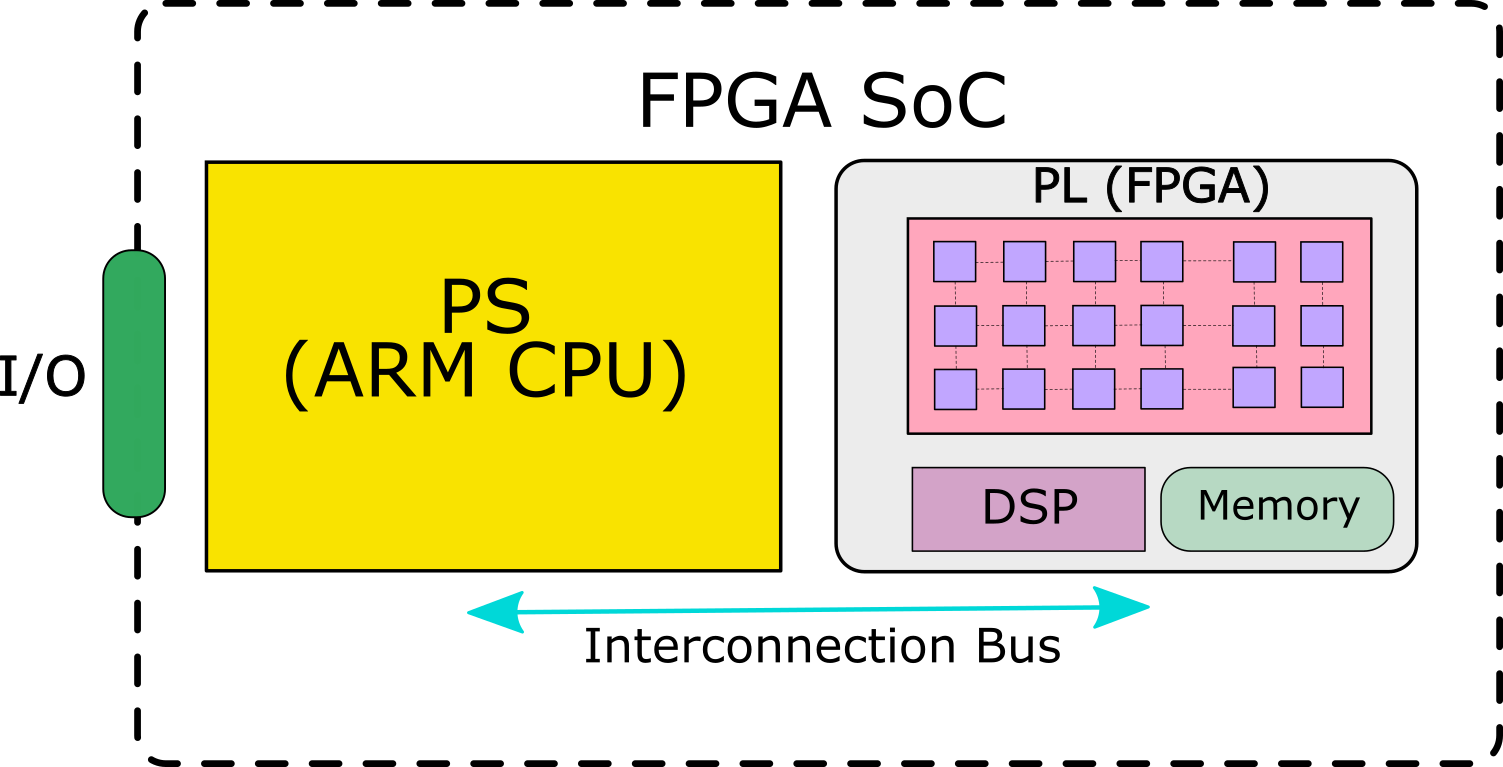
\includegraphics[width=0.6\textwidth]{FPGA_SoC.png}
    \caption{Arquitectura típica de un FPGA SoC.}
    \label{fig:fpga_soc}

\end{figure}

\subsection{Procesamiento Digital de Pulsos}
 
\noindent Como se explicó en el apartado de electrónica de front-end, los filtros analógicos suelen aplicar una combinación de diferenciaciones e integraciones de la forma de onda de voltaje para transformarla en una forma similar a la de una gaussiana, cuya amplitud es proporcional al voltaje $V$ y, por lo tanto, a la energía de la radiación. Sin embargo, de acuerdo a \cite{loudenuclearspectroscopy}, en el enfoque digital, tras la digitalización de la señal utilizando un ADC, se aplica un filtro matemático a esta serie de valores digitales para eliminar los componentes de ruido de alta frecuencia, mejorando así la SNR y determinando la amplitud de voltaje $V$.\\

\noindent Este enfoque presenta ventajas significativas en comparación con el procesamiento de señales analógicas tradicional, entre las cuales destacan \cite{radeka1968optimum}:

\begin{itemize}
    \item Aplicación de análisis considerando diferencias pulso a pulso: Permite analizar cada pulso individualmente, teniendo en cuenta sus particularidades.
    \item Análisis de señales de carga inducida transitoria: Facilita la interpretación de señales transitorias que pueden ser difíciles de captar con métodos analógicos.
    \item  Mejora del parámetro de tiempo muerto: Reduce las limitaciones temporales que pueden afectar la adquisición continua de señales.
    \item Captura fácil de señales, incluida la implementación de análisis complejos: Simplifica la adquisición de datos y permite realizar análisis detallados y sofisticados.
    \item Procesamiento de señales con criterios basados en coincidencias (diferentes detectores o diferentes partes del mismo detector): Facilita la correlación de eventos entre múltiples detectores o áreas de un detector.
    \item Aplicación efectiva de post-procesamiento de datos: Permite el pre-análisis de formas de onda, modelado de pulsos y verificación de algoritmos de deconvolución de superposición de pulsos (pulse pile-up).

\end{itemize}

\noindent La implementación de procesadores digitales de pulsos (DPP) en FPGA, gracias a su riqueza en recursos lógicos digitales, les permite soportar múltiples modos de adquisición, como análisis de altura de pulso, escalado de canales múltiples, escalado de espectros múltiples y adquisición en modo de lista con marcas de tiempo. Además, ofrecen funcionalidades muy especializadas como discriminación y corrección de la forma del pulso, rechazo de superposición de pulsos (pulse pile-up), conteo sin pérdidas y otras características que respaldan la medición. Adicionalmente, múltiples DPP pueden operar de manera sincronizada para permitir la correlación temporal de eventos provenientes de múltiples fuentes de señal, como detectores separados o segmentos de un mismo detector. \\

\noindent En el capítulo System, se desarrolla la aplicación de los conceptos expuestos en este capítulo, en un sistema experimental de lectura y procesamiento para detectores GEM.

\noindent Como se expuso anteriormente, los electrones multiplicados son recogidos en los electrodos de salida del GEM, resultando una señal de corriente eléctrica que puede ser medida y analizada. Dependiendo de los objetivos del experimento, distintas etapas electrónicas pueden ser implementadas a continuación. Sin embargo, el objetivo de estas converge a preservar y transportar la información física de interés contenida en la señal, optmizando factores clave como \cite{knoll2010radiation}:

\begin{itemize}
    \item Supresión de ruido 
    \item Reducción del tiempo muerto
    \item Reducción del déficit balístico para mejorar la resolución y reducir la distorsión de los picos
\end{itemize}

\noindent Aunque los distintos tipos de detectores generan señales eléctricas únicas, dependiendo de los procesos físicos que ocurren en su interior, es posible identificar características comunes que facilitan la comprensión de conceptos clave en el acondicionamiento y procesamiento de señales.

%Particularmente en la medición de eventos propios de cor´pusculos, se presentan señales de tipo pulsado...
\section{Montaje Experimental}
\section{Resultados}
\section{Análisis y conclusiones}

\bibliographystyle{ieeetr}
\bibliography{references}
\end{document}